\chapter{Word Embedding}
Word embeddings is distributed representation of words in a vector space. With the learning algorithm it can capture the contextual or co-occurrence information. The word embedding has an interesting and important property: similar words will have similar distribution in the embedding space, with that property, we can find meaningful near-synonyms or  Some successful methods for learning word embedding like word2vec\cite{mikolov2013distributed}, \cite{pennington2014glove}

\section{Monolingual Embedding}
\begin{figure}[h]
	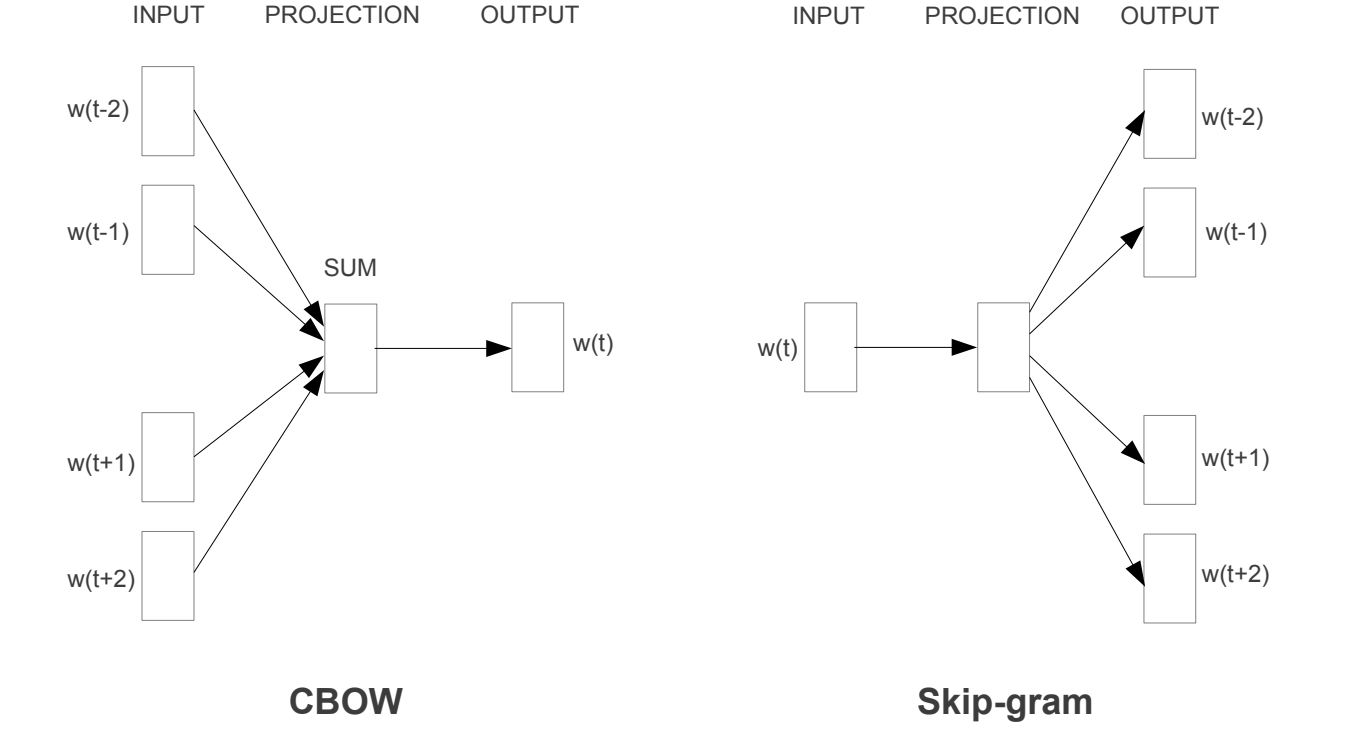
\includegraphics[width=12cm]{word2vec}
	\caption{Global attention model (\cite{mikolov2013efficient})}
	\centering
\end{figure}
\subsection{CBOW and Skip-gram Model}
CBOW model and skip-gram model are currently mainstream neural network to learn the word embedding. Algorithmically,  CBOW tries to predict the current word based on the context while skip-gram model tries to maximize classification of a word based on another word in the same sentence. Using skip-gram model as example, given a large training corpus represented as a sequence of words ${w_1, \cdots w_N}$, the objective of the model is to maximize the following log-likelihood:
\[ \sum_{s=1}^{N} \sum_{w_t \in \mathcal{C}_s} \log\ {p(w_t|w_s)} \]
where $w_s$ is the current word, the context $\mathcal{C}^s$ is the set of words surrounding word $w_s$, so $w_t$ means the word to predict. So probability above can be interpreted as observing a context word $w_t$ given $w_s$.\\

Suppose we can given a scoring function s which maps word pairs to score in $\mathbb{R}0$ like cosine similarity, the probability can be defined like softmax function:
\begin{align}
p(w_t | w_s) & = \textrm{softmax} {(s(w_t, w_s))} \\
& = \frac{\exp\{s(w_t, w_s)\}}{\sum_{w^{\prime} \in W}{\exp\{s( w^{\prime}, w_s)\}}} 
\end{align}
where $W$ is the whole vocabulary. \\

We train the model by maximizing its log-likelihood on the training dataset, i.e. by maximizing:
\begin{align}
J_{ML} & = \log p(w_t| w_s)	\\
& = s(w_t, w_s) - \log(\sum_{w^\prime \in W} {\exp\{s(w^\prime, w_s)\}})	
\end{align}

\textbf{Noise-Contrastive Training}\\
However the normalization on the whole vocabulary is very expensive since it is conducted for all words at every training step. The problem of predicting words can be considered as an independent binary classification task. For example in the skip-gram model, we consider all the context words as positive samples and the words randomly sampled from the dictionary as the negative ones. Then the training objective is 
\[J_{NEG} = \log {Q_{\theta}{(D=1 | w_t, w_s)}} + \sum_{w^{\prime} \sim P_{noise}} {\log{Q_{\theta}{(D=0 | w^{\prime}, w_s )}}}  \]

where ${Q_{\theta}{(D=1| w_t, w_s)}}$ is the binary logistic regression probability. In practice, we draw k contrastive words from the noise distribution. Then the model are instead trained to discriminate the read target word $w_t$, from imaginary (noise) words. Since we only calculate the loss function for k samples instead the whole vocabulary, it becomes much faster to train.\\
According to  empirical results, CBOW works better on smaller datasets because CBOW smoothes over a lot of the distributional information while Skip-Gram model performs better when we have larger datasets



\subsection{FastText}
The training methods above treat each word as a distinct word embedding, however intuitively we can obtain more information from the morphological information of words. A subword model was proposed to try to fix such problem.The training network is similar, the model design a new presentation of the word: it adds speicial symbols $<$, ${>}$ as boundary information at the beginning and the end of a word. Then a normal word is represented as a bag of character $n$-grams . For example the word "where" and n equals 3, the it can be represented as the following 5 tri-grams: 
\[ <wh, whe, her, ere, re>\]
Suppose in this way we denote a word ${w}$ as ${G_{w}}$ the set of character ${n}$-grams, we assign for each character ${n}$-gram $g$ in ${G_{w}}$, we assign a distinct vector $z_g$, we will finally represent the embedding of word ${w}$ as the sum of these vector and also for the scoring function:
\[s(w, w_s) = \sum_{g \in G_{w}} z_g^{T} w_s \]
	
\section{ Cross-lingual Word Embedding}



	Cross-lingual word embedding is defined as word embedding of multiple languages in a joint embedding space. Mikolov first notice that the embedding distributions exhibit similar structure across languages. They proposed to use a linear mapping from the source embedding to target embedding. \\
	\begin{figure}[t]
		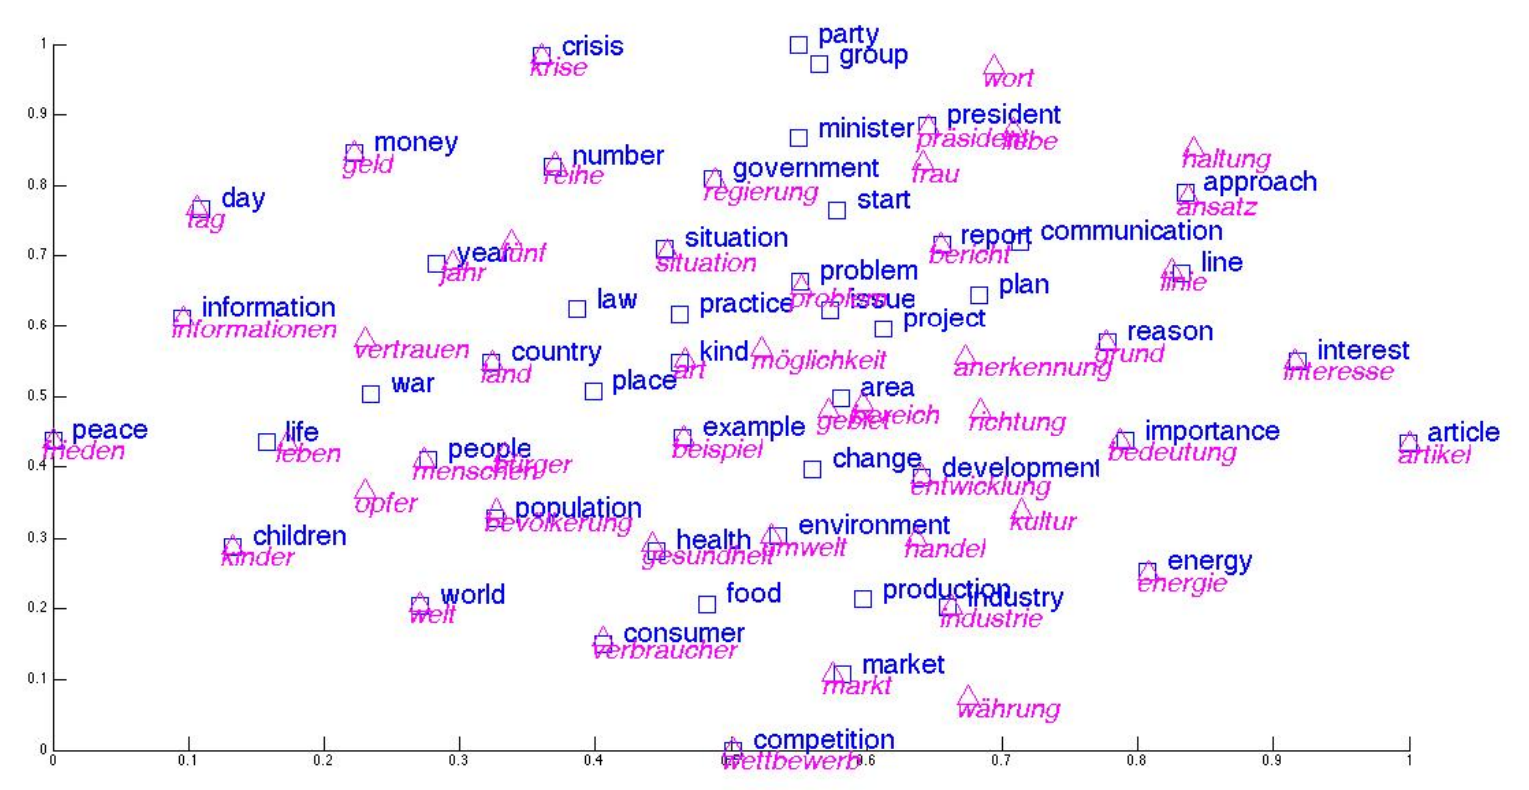
\includegraphics[width=14cm]{crossembedding}
		\centering
		\caption{A cross-lingual embedding space between German and English (\cite{ruder2017survey})}
	\end{figure}
	
	Cross-lingual word embeddings are appealing due to two main factors: they enable not only cross-lingual semantics, reasoning about word meaning in multilingual contexts, for example, we can induce the bilingual dictionary by calculating the cross-lingual word similarities, but also knowledge transfer between languages, most importantly between rich-resource and lean-resource languages (\cite{adams2017cross}). 

	In the thesis, I assume there are two set of embeddings ${e}$, ${f}$trained separately on monolingual data.  The propose of cross-lingual word embedding training is to learn such a mapping ${W \in }$ from source embedding space to target embedding space, so $Wf_i, e_j$ in the same embedding space and for all corresponding word pairs, we need to optimize the mapping ${W}$, so that"
	 
	
	\[ \arg\min_{W \in R^{d \times d}} \sum_{i} \lVert Wf_i - e_i \rVert \]
	where $d$ is the dimension of embeddings, and the distance ${\lVert Wf_i - e_i \rVert}$ can be different types. We prefer the Euclidean distance.  

first observe that word embeddings trained separately on monolingual corpora exhibits isomorphic structure across languages, as illustrated in Figure {}. That means we can create a connection between source embedding and target embedding even with simple linear mapping. This has far-reaching implication on low-resource scenarios {}{}{}, because word embedding requires only plain text to train, which is the most abundant form of linguistic resource.
	

\subsection{Training Algorithm}
Most training methods can be divided into joint training approaches and mapping-based approaches. , .   first train monolingual word representations on corresponding corpus separately. Then mappings are learned to project different embeddings into the shared space. They learn the transformation from word alignments or bilingual dictionaries. Some works focus on learning the mapping from the source embedding space to the target embedding space. The criterion is to minimize the mean squared error between the transformed source embeddings and the target embeddings. Another type like CCA-based mapping use canonical correlation analysis (CCA) to project words from two languages into a shared embedding space (). \\
\textbf{Joint Training Approaches}\\
Joint training means to optimize the source and target embeddings objectives $\mathcal{L(\cdot)}$ jointly with the cross-lingual regularization term $\Omega(\cdot)$. 
\[ \mathcal{L} =  \mathcal{L}_{\text{skip-gram}}^e + \mathcal{L}_{\text{skip-gram}}^f + \lambda \cdot \Omega(\cdot)  \]
where the first two losses are exact the same as those in monolingual embedding training. While the $\Omega(\cdot)$  encourages the similar words representations to be similar for words that are related across different languages.

Different cross-lingual regularization terms are proposed to optimize the cross-lingual embeddings (\cite{coulmance2016trans}, \cite{luong2015bilingual}, \cite{gouws2015bilbowa}). For example, \cite{gouws2015bilbowa} models it as: 
\[ \Omega_{\text{BilBOWA}} = {\lVert \frac{1}{I}  \sum_{e_i \in e_1^I} \bm{e}_i - \frac{1}{J} \sum_{f_j \in f_1^J} \bm{f}_j\rVert}^2 \]
where $\bm{f}_j$ and $\bm{e}_i$ are the word embeddings for words in parallel source and target sentences. Instead of relying on expensive word alignments which minimize the distance that aligned to each other, they minimize the distance between the mean of the word representations in the aligned sentences. 

\textbf{Mapping-based Approaches}: \\
First train monolingual word embeddings independently on large monolingual corpora and then find the most suitable transformation matrix that maps the embeddings into a shared embedding space. The mapping is trained based on bilingual dictionary.

Multilingual learning can be categorized into mapping-based approaches and regularization-based approaches. In the mapping-based approaches, the embedding is performed for each language individually with monolingual data, and then the mapping are learned using multilingual data to represent the relation between the languages. One method is to learn the linear mapping projection, another is to learn mappings that project word vectors of all languages to a common low-dimension space, where the correlation of the multilingual word pairs is maximized with the canonical correlation analysis (CCA). The advantages of approach is that it is very fast to learn the embedding alignments. The main draw back of this approach is that it is not clear if a single transformation whether linear or nonlinear can capture the relationship between all words in different languages.

The regularization-based approaches involve the multilingual constraint in the objective function for learning the embedding, adds an extra term that reflects the distances of some pairs of semantically related words from different languages into the objective function. 

\subsubsection{Canonical Correlation Analysis (CCA)}

let $E \in \mathbb{R}^{m \times d_1}$ and $F \in \mathbb{R}^{n \times d_2}$ be word embeddings of two different vocabularies where rows represent words. Since the two vocabularies are of different sizes and there might be not exist translation of every word. Let $\bm{e}$,$\bm{f}$ be two corresponding vectors from , and be the two projection directions. Then the projected vectors are:
\[ \] 
and the correlation between the projected vectors can be written as:
 \[\rho(\bm{f}^{\prime}, \bm{e}^{\prime}) = \frac{\mathbb{E[(\bm{f})(\bm{e})]}}{\sqrt{\mathbb{E[(\bm{f})^2]} \sqrt{\bm{E(\bm{e})^2}}}}\] 
 \[ \frac{\bm{u}^T\Sigma_{fe} \bm{v}}{\sqrt{\bm{u}^T \Sigma_{ff}\bm{u}} \sqrt{\bm{v}^T\Sigma_{ee}\bm{v}}} \]
 
 where $\Sigma_P{fe}$ and $\Sigma_{ff}$ are the cross-view and within 
 
 CCA maximizes $\rho$ for the given set of vectors ${}$ and ${}$ and outputs two projection matrix :
 
 Using these two prokection vectors we can project the entire vocabularies of the two languages  
 
 
\textbf{Deep Canonical Correlation Analysis}
A linear feature mapping is often not sufficiently powerful to faithfully capture the hidden, non-linear relations within the data. proposed a non-linear extension of CCA using deep neural networks. In this model, two neural networks are used to extract features from each voew, and trained to maximize the correlations between outputs in the two views, measured by a linear CCA steo with projection mappings the neural network weights and linear projections are optimized together using the objective 
\[ \]
%where $W_f$ and $W_e$ are the weights of the two networks and ${}$ ${}$, ${}$ are covariance matrices computed for   in the ssame way as CCA. The final transformation is the composition of the neural network ans CCA projection, $\bm{u}^T \bm{f}$ for the view. The algorithm does not have a closed-form solution but the parameters can be learned via gradient-based optimization with mini-batch stochastic gradient descent .
%\begin{enumerate}
%	\item Mapping based approaches\\
%	First train the monolingual word embedding separately and then seek the seed dictionary to learn the mapping. 
%	\item Pseudo-multi-lingual corpora-based approaches\\
%	Use the monolingual embedding training method on constructed corpora that contains both the source and the target language.
%	\item Joint methods\\
%	Take the parallel text as input and minimize the source and target language losses jointly with the cross-lingual regularization term
%\end{enumerate}


The joint formulation of the learning objective provided as:
\[ J = \mathcal{L}^s + \mathcal{L}^t + \Omega(s,t) \]
where ${\mathbb{L}^s}$ and ${\mathbb{L}^t}$ are monolingual objectives in each language optimized jointly with the cross-lingual regularization objective.

exact cross-lingual objective as follows:
\begin{align*}
	 \Omega(E, F) = & \sum_{i} \sum_{j} a_{ij} {\lvert \bm{e}_i - \bm{f}_j \rvert}^2 \\
	= & (E - F)^2 A (E - F)
\end{align*}
where subscript A indicates that the alignments are fixed. A captures the relationships between all source and target vocabularies.

A dictionary is necessary for learning the cross-lingual word embedding. 
minimizing the distance in a bilingual dictionary.\\

Xing \cite{ } showed that the results are improved when we constrain the ${W}$ to be an orthogonal matrix. This constraint,  the optimal transformation can be efficiently calculated in linear time with respect to the vocabulary size.

The problem then is simplified as the Procrustes problem and there exists a closed-form solution obtained from the SVD of ${EF^T}$

\textbf{Orthogonal Constraints}
Starting from \cite{mikolov2013exploiting}, the mapping from source embedding space to target embedding space can be represented as a linear repression. The objective can be defined as:
\[ \min_{W} \sum_{i} {\lvert Wf - e  \rVert}^2 \]
Since we retrieve the word translation according to cosine similarity, it's better to solve the problem by redefine the optimization function using the cosine distance:
\[ \argmax{W} {\sum_{i} (W f_i)^T e^i} \]. We consider the source and target embedding in the same space. In this case, the normalization constraint on word vectors can be satisfied by constraining $W$ as an orthogonal matrix. 
This is equivalent to minimizing the (squared) Frobenius norm of the residual matrix:
\[ W^* = \argmin{W} {\lVert WF - E \rVert}^2_F \]
The problem boils down to the Procrustes problem which has a closed form solution obtained from the singular value decomposition (SVD).
\[W* = = UV^T , \quad U\Sigma V^T = SVD(EF^T) \]
\textbf{CSLS Loss}
Inspired from the work of \cite{conneau2017word}, where the dictionary inducted from CSLS loss: ${\bm{e}}$
\[ CSLS(\bm{e} ,\bm{f}) = -2 cos(\bm{e}, \bm{f}) + \frac{1}{k} \sum_{\bm{e}^{\prime} \in N_{\bm{e}}(\bm{f})} {cos(\bm{e}^{\prime}, \bm{f})}+ \frac{1}{k}  \sum_{\bm{f}^{\prime} \in N_{\bm{f}}(\bm{e})   } {cos(\bm{f}^{\prime}, \bm{e})}\]
since we have ${cos(\bm{We}, \bm{f}) = \bm{e}^T \bm{W}^T \bm{f}}$

The loss function can be rewritten as:
\[ \min_{\bm{W} \in } = \frac{1}{n} \sum_{i=1}^{n} \]


Minimization of a non-smooth cost function over the manifold of orthogonal matrices . Instead of using manifold optimization tools, \cite{bibid} proposed to derive convex relaxations that can lead to a simple and tractable minimization algorithm.
\begin{itemize}
	\item Spectral norm:
	replacing the set of orthogonal matrices $1$ by its convex hull, that is the set of matrices with singular values smaller than 1, the unit ball of the spectral norm 
	\item Frobenius norm:
	replacing the the set of orthogonal matrices $1$ with ball of radium $\sqrt{d}$ in Frobenius norm
\end{itemize}
 
With such two relaxations, the CSLS loss is constrained to a convex function with respect to the mapping $\bm{W}$.

We train the linear mapping with in the spectral norm by projected gradient descent:$2$ 
For each iteration, train the mapping $\bm{W}$ with gradient descent, then constrain the mapping by projection of the set.
\begin{itemize}
	\item Spectral norm\\
	take the SVD of the trained matrix, threshold the singular values to one
	\item Probenius norm\\
	divide the matrix by its Frobenius norm
\end{itemize} 



	
	